\documentclass[fleqn]{article}
\oddsidemargin 0.0in
\textwidth 6.0in
\thispagestyle{empty}
\usepackage{import}
\usepackage{amsmath}
\usepackage{graphicx}
\usepackage{flexisym}
\usepackage{calligra}
\usepackage{amssymb}
\usepackage{bigints} 
\usepackage[english]{babel}
\usepackage[utf8x]{inputenc}
\usepackage{float}
\usepackage[colorinlistoftodos]{todonotes}


\DeclareMathAlphabet{\mathcalligra}{T1}{calligra}{m}{n}
\DeclareFontShape{T1}{calligra}{m}{n}{<->s*[2.2]callig15}{}
\newcommand{\scriptr}{\mathcalligra{r}\,}
\newcommand{\boldscriptr}{\pmb{\mathcalligra{r}}\,}

\definecolor{hwColor}{HTML}{442020}

\begin{document}

  \begin{titlepage}

    \newcommand{\HRule}{\rule{\linewidth}{0.5mm}}

    \center

    \begin{center}
      
\includegraphics[height=11cm, width=11cm]{asu.png}
    \end{center}

    \vline

    \textsc{\LARGE Classical Parts/Field/Matter III}\\[1.5cm]

    \HRule \\[0.5cm]
    { \huge \bfseries Midterm Exam 1}\\[0.4cm] 
    \HRule \\[1.0cm]

    \textbf{Behnam Amiri}

    \bigbreak

    \textbf{Prof: Samuel Teitelbaum}

    \bigbreak

    \textbf{{\large \today}\\[2cm]}

    \vfill

  \end{titlepage}


  \begin{itemize}
    \item This exam is available all weekend, but should take you 4-6 hours to complete.
    \item Your solutions must be uploaded to Canvas just as you do with homework.
    \item The exam should be taken without the use of internet (aside from Canvas materials, and email
    in the event that you have questions during the exam).
    \item The only allowed materials are: Griffiths textbook, your math methods textbook, any materials
    on Canvas, and your own hand-written or hand-typed notes.
    \item Do not discuss the midterm problems with anyone until after Febuary $23, ~ 2022$.
    \item If you get stuck on math, explain the physics as well as you can.
  \end{itemize}

  \pagebreak

  \textbf{Vector Calculus Identities}

  \vspace{1cm}

  $
    \begin{cases}
      \nabla \times \left(\nabla V\right)=0
      \\
      \\
      \nabla.\left(\nabla \times \overrightarrow{A}\right)=0
      \\
      \\
      \nabla \times \left(\nabla \times \overrightarrow{A}\right)=\nabla\left(\nabla \overrightarrow{A}\right)-\nabla^2 \overrightarrow{A}
      \\
      \\
      \nabla^2 \overrightarrow{A}=\nabla^2 A_x ~ \hat{x}+\nabla^2 A_y ~ \hat{y}+\nabla^2 A_z ~ \hat{z}
      \\
      \\
      C=A+i ~ B=r ~ e^{i \phi}
      \\
      \\
      Re(C)=A=r ~ cos(\phi)
      \\
      \\
      Im(C)=B=r ~ sin(\phi)
      \\
      \\
      |C|=r=\sqrt{A^2+B^2}
    \end{cases}
  $

  \pagebreak

  \begin{enumerate}
    \item \textbf{Problem 1 [20 points]}
    \begin{enumerate}
      \item Derive the charge continuity equation directly from Maxwell’s equations (7.40).

        \textcolor{hwColor}{
          \\
          From page $337$ of the textbook we have the Maxwell’s equations (E.g $ ~ 7.40$) as
          $
            \\
            \\
            \begin{cases}
              \text{Gauss’s law}: ~~~ \nabla.E=\dfrac{1}{\epsilon_0} \rho
              \\
              \\
              \text{No name}: ~~~ \nabla.B=0
              \\
              \\
              \text{Faraday’s law}: ~~~ \nabla \times E=-\dfrac{\partial B}{\partial t}
              \\
              \\
              \text{Ampère’s law with Maxwell’s correction}: ~~~ \nabla \times B=\mu_0 ~ J+\mu_0 ~ \epsilon_0 ~ \dfrac{\partial E}{\partial t}
            \end{cases}
            \\
            \\
          $
          \emph{If the charge in some region changes, then exactly that amount of charge must have passed in or out through the surface.} We 
          know that current density is $J=\dfrac{I}{A}$ and volume charge density is $\rho=\dfrac{Q}{V}$. Also we know that 
          $ 
            \\
            \\ 
            Q_{in}+Q_{out}=Constant \Longrightarrow \dfrac{d Q_{in}}{dt}+\dfrac{d Q_{out}}{dt}=0
            \\
            \\
            \therefore ~~~ \dfrac{d Q_{in}}{dt}=-\dfrac{d Q_{out}}{dt} ~~~~ \checkmark
            \\
            \\
            \\
            Q(t)=\bigints\limits_{V} ~ \rho(r,t) ~ d\tau
            \Longrightarrow
            \dfrac{dQ}{dt}=-\bigoint\limits_{V} J.da
            \\
            \\
            \\
            \bigints\limits_{V} ~ \dfrac{\partial \rho}{\partial t} ~ d\tau=-\bigints\limits_{V} ~ \nabla.J ~ d\tau
            \\
            \\
            \\
            \therefore ~~~ \boxed{
              \dfrac{\partial \rho}{\partial t}=-\nabla.J
            } ~~~~ \checkmark
            \\
            \\
            \\
          $
          This is the continuity equation—the precise mathematical statement of local conservation of charge. Starting
          from the Ampère’s law we have.
          \\
          \\
          $
            \nabla \times B=\mu_0 ~ J+\mu_0 ~ \epsilon_0 ~ \dfrac{\partial E}{\partial t}
            \\
            \\
            \\
            \nabla.\left[\nabla \times B\right]=\nabla.\left[\mu_0 ~ J+\mu_0 ~ \epsilon_0 ~ \dfrac{\partial E}{\partial t}\right]
            \\
            \\
            \\
            0=\nabla.\left(\mu_0 ~ J\right)+\nabla.\left(\mu_0 ~ \epsilon_0 ~ \dfrac{\partial E}{\partial t}\right)
            =\mu_0 \left[
              \nabla.J+\nabla.\left(\epsilon_0 ~ \dfrac{\partial E}{\partial t}\right)
            \right]
            \\
            \\
            \\
            0=\nabla.J+\nabla.\left(\epsilon_0 ~ \dfrac{\partial E}{\partial t}\right)
            =\nabla.J+\epsilon_0 ~ \left(\nabla.\dfrac{\partial E}{\partial t}\right)
            =\nabla.J+\epsilon_0 ~ \dfrac{\partial}{\partial t} \left(\nabla.E\right)
            \\
            \\
          $
          Gauss’s law states $\nabla.E=\dfrac{1}{\epsilon_0} \rho$, hence we have:
          \\
          \\
          $
            0=\nabla.J+\epsilon_0 ~ \dfrac{\partial}{\partial t} \left(\dfrac{1}{\epsilon_0} ~ \rho\right)
            =\nabla.J+\dfrac{\partial \rho}{\partial t}
            \\
            \\
            \\
            \therefore ~~~ \boxed{
              \dfrac{\partial \rho}{\partial t}=-\nabla.J
            } ~~~~ \checkmark
            \\
            \\
          $
        }
      
      \item Suppose there is a charge current density $\mathbf{J}=Cx ~ \hat{x}$ within some region of space. Find the
      charge density $\rho(r, t)$ at the origin $r=0$ at some later time $t$, assuming that $\rho(0, 0)=0$.

        \textcolor{hwColor}{
          \\
          At the origin $r=0 ~ (r=x ~ \hat{x}+y ~ \hat{y}+z ~ \hat{z})$. Using the continuity equation we have:
          \\
          \\
          $
            \dfrac{\partial \rho}{\partial t}=-\nabla.J=-\left[\nabla. \left(Cx ~ \hat{x}\right)\right]
            =-\left[\dfrac{\partial}{\partial x} ~ \hat{x}. \left(Cx ~ \hat{x}\right)\right]
            \\
            \\
            \\
            \therefore ~~~ \dfrac{\partial \rho}{\partial t}=-C 
            \Longrightarrow \bigints \dfrac{\partial \rho}{\partial t} ~ dt
            =\bigints -C ~ dt
            \\
            \\
            \\
            \therefore ~~~ \boxed{
              \rho(0,t)=-Ct 
            } ~~~~ \checkmark
          $
          \\
          \\
        }
      
    \end{enumerate}


    \item \textbf{Problem 2 [20 points]} A toroid with a current $I$ and a total of n windings is placed in an uniform
    electric field $\mathcal{E}=E ~ \hat{z}$, which points along the axis of symmetry of the toroid. The toroid has a radius
    and rectangular cross section of dimensions shown in the figure.

      \begin{figure}[h!]
        \centering
        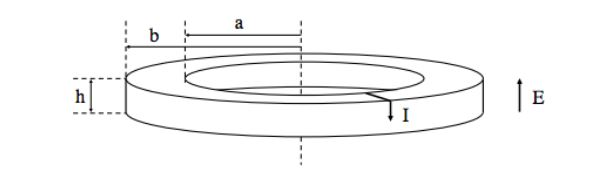
\includegraphics[height=4cm, width=8cm]{One.JPG}
      \end{figure}

      \begin{enumerate}
        \item Determine the Poynting vector everywhere in space. Use the standard cylindrical coordinates
        with axes $\hat{s}$, $\hat{\phi}$, $\hat{z}$.

          % \textcolor{hwColor}{
          %   \\
          % }

        \item Determine the total flux of field energy into the toroid by integrating the Poynting vector.

          % \textcolor{hwColor}{
          %   \\
          % }

        \item Determine the total linear momentum stored in the fields.

          % \textcolor{hwColor}{
          %   \\
          % }

        \item Determine the total angular momentum stored in the fields.

          % \textcolor{hwColor}{
          %   \\
          % }

        \item Qualitatively, what happens to the toroid when the E field is reduced to zero?

          % \textcolor{hwColor}{
          %   \\
          % }

      \end{enumerate}

    \pagebreak

    \item \textbf{Problem 3 [20 points]} 
    Two infinite, electrically neutral wires are parallel to each other and each carries a current $I$ flowing
    in the $\hat{z}$ direction. The axes of the wires pass through the points $\pm d\hat{x}$ (hence they are separated by
    a distance $2d$).
    \begin{enumerate}
      \item Determine the force per unit length acting on the wire passing through $+d\hat{x}$ by making use of
      the Maxwell stress tensor. Make sure that you get the correct direction of the force.

        \textcolor{hwColor}{
          \\
          On page 364 of the textbook we learned that the total electromagnetic force on the charges in $\mathcal{V}$ is
          \\
          \\
          $
            F=\bigoint\limits_{S} \overleftrightarrow{T}.da-\epsilon_0 \mu_0 \dfrac{d}{dt} \bigints\limits_{v} S d\tau
          $
          \\
          \\
          The \textbf{Maxwell Stress Tensor} is defined as 
          \\
          \\
          $
            T_{ij} \equiv \epsilon_0 \left(E_i E_j - \dfrac{1}{2} \delta_{ij} E^2 \right)
            +\dfrac{1}{\mu_0} \left(B_i B_j - \dfrac{1}{2} \delta_{ij} B^2\right) ~~~~~~~ \delta_{ij}=\begin{cases}
              1 ~~~~ \text{if} ~~ i=j
              \\
              0 ~~~~ \text{if} ~~ i \neq j
            \end{cases}
            \\
            \\
            \\
            \begin{cases}
              T_{xx}=\dfrac{\epsilon_0}{2} \left(E_x^2-E_y^2-E_z^2\right)+\dfrac{1}{2 \mu_0} \left(B_x^2-B_y^2-B_z^2\right)=\dfrac{1}{2 \mu_0} B_x^2
              \\
              \\
              T_{yy}=\dfrac{\epsilon_0}{2} \left(E_y^2-E_z^2-E_x^2\right)+\dfrac{1}{2 \mu_0} \left(B_y^2-B_z^2-B_x^2\right)=-\dfrac{1}{2 \mu_0} B_x^2
              \\
              \\
              T_{zz}=\dfrac{\epsilon_0}{2} \left(E_z^2-E_y^2-E_x^2\right)+\dfrac{1}{2 \mu_0} \left(B_z^2-B_y^2-B_x^2\right)=-\dfrac{1}{2 \mu_0} B_x^2
              \\
              \\
              T_{xy}=T_{yx}=\epsilon_0 \left(E_x E_y\right)+\dfrac{1}{\mu_0} \left(B_x B_y\right)=0
              \\
              \\
              T_{yz}=T_{zy}=\epsilon_0 \left(E_y E_z\right)+\dfrac{1}{\mu_0} \left(B_y B_z\right)=0
              \\
              \\
              T_{zx}=T_{xz}=\epsilon_0 \left(E_z E_x\right)+\dfrac{1}{\mu_0} \left(B_z B_x\right)=0
            \end{cases} ~~~~~ \checkmark
            \\
            \\
            \\
          $
          \\
          \\
        }

        % \overleftrightarrow{T}

      \item Confirm the result in part (a) by doing the easier calculation (i.e. use the Lorentz force law).
      The following integral might be helpful for part (a):
      $$
        \int\limits_{-\infty}^{+\infty} ~ \dfrac{y^2}{\left(y^2+d^2\right)^2} ~ dy=\dfrac{\pi}{2d} 
      $$

        % \textcolor{hwColor}{
        %   \\
        % }

    \end{enumerate}

    \item \textbf{Problem 4 [20 points]} The electric field of an elliptically polarized EM wave in vacuum is formed by the superposition
      $$
        E(r,t)=E_y ~ sin(ax-\omega t) ~ \hat{y}+E_z ~ cos(ax-\omega t) ~ \hat{z}
      $$
      where $a$ is a positive constant.
      \begin{enumerate}
        \item What is the direction that the wave travels, and what is its wavelength?

          \textcolor{hwColor}{
            \\
            Based on the given wave, we can see that one wave is in the y-direction and the other one is in the z-direction. We learn that
            the direction of propagation is in the direction of $E \times B$ (\emph{the Poynting vector points in the direction of the propagation of the wave})
            therefore, the direction that the wave tarvels is in the x-direction.
            \\
            From page 387 of the textbook we learned that when two waves have the same frequency and wave number (constructive)
            then the \emph{combined wave still has the same frequency and wavelength}.
            \\
            For a wave with $A ~ cos\left[k\left(a-vt\right)+\delta\right]$ format, the wavelength is found by $\lambda=\dfrac{2\pi}{k}$.
            \\
            \\
            $
              \therefore ~~~ \lambda=\dfrac{2\pi}{1} \Longrightarrow \boxed{\lambda=2\pi} ~~~~ \checkmark
            $
          }

        \item Determine the radiation pressure carried by the field by deriving the Maxwell stress tensor for
        the field.

          \textcolor{hwColor}{
            \\
            In chapter 8, we learned about the \textbf{Maxwell stress tensor}. Let's rewrite again here. Note the  \textbf{Kronecker delta},
            $\delta_{ij}$ is $1$ if the indices are the same $(\delta_{xx}=\delta_{yy}=\delta_{zz}=1)$ and zero otherwise
            $(\delta_{xy}=\delta_{xz}=\delta_{yz}=0)$. Also, $c^2=\dfrac{1}{\mu_0 ~ \epsilon_0}$ comes from the wave equation that  
            can be derived from Maxwell's equations.
            \\
            \\
            $
              T_{ij} \equiv \epsilon_0 \left(E_i ~ E_j -\dfrac{1}{2} \delta_{ij} ~ E^2 \right)
              +\dfrac{1}{\mu_0} \left(B_i ~ B_j -\dfrac{1}{2} \delta_{ij} B^2 \right) ~~~~~~~~~~~~~~~ (8.17)
              \\
              \\
              \\
              \begin{cases}
                T_{xx}=\dfrac{\epsilon_0}{2} \left(E_x^2-E_y^2-E_z^2\right)+\dfrac{1}{2 \mu_0} \left(B_x^2-B_y^2-B_z^2\right)
                \\
                \\
                T_{yy}=\dfrac{\epsilon_0}{2} \left(E_y^2-E_z^2-E_x^2\right)+\dfrac{1}{2 \mu_0} \left(B_y^2-B_z^2-B_x^2\right)
                \\
                \\
                T_{zz}=\dfrac{\epsilon_0}{2} \left(E_z^2-E_y^2-E_x^2\right)+\dfrac{1}{2 \mu_0} \left(B_z^2-B_y^2-B_x^2\right)
                \\
                \\
                T_{xy}=T_{yx}=\epsilon_0 \left(E_x E_y\right)+\dfrac{1}{\mu_0} \left(B_x B_y\right)
                \\
                \\
                T_{yz}=T_{zy}=\epsilon_0 \left(E_y E_z\right)+\dfrac{1}{\mu_0} \left(B_y B_z\right)
                \\
                \\
                T_{zx}=T_{xz}=\epsilon_0 \left(E_z E_x\right)+\dfrac{1}{\mu_0} \left(B_z B_x\right)
              \end{cases}
              \\
              \\
            $
            \\
            Since $B=0$ we have
            \\
            \\
            $
              \\
              \begin{cases}
                T_{xx}=\dfrac{\epsilon_0}{2} \left(E_x^2-E_y^2-E_z^2\right)
                =-\dfrac{\epsilon_0}{2} \left(E_y^2+E_z^2\right)
                \\
                \\
                T_{yy}=\dfrac{\epsilon_0}{2} \left(E_y^2-E_z^2-E_x^2\right)
                =\dfrac{\epsilon_0}{2} \left(E_y^2-E_z^2\right)
                \\
                \\
                T_{zz}=\dfrac{\epsilon_0}{2} \left(E_z^2-E_y^2-E_x^2\right)
                =\dfrac{\epsilon_0}{2} \left(E_z^2-E_y^2\right)
                \\
                \\
                T_{xy}=T_{yx}=\epsilon_0 \left(E_x E_y\right)=0
                \\
                \\
                T_{yz}=T_{zy}=\epsilon_0 \left(E_y E_z\right)
                \\
                \\
                T_{zx}=T_{xz}=\epsilon_0 \left(E_z E_x\right)=0
              \end{cases}
              \\
              \\
              \\
              \overleftrightarrow{T}=\begin{pmatrix}
                T_{xx} & T_{xy} & T_{xz} 
                \\
                T_{yx} & T_{yy} & T_{yz} 
                \\
                T_{zx} & T_{zy} & T_{zz} 
              \end{pmatrix}=\begin{pmatrix}
                -\dfrac{\epsilon_0}{2} \left(E_y^2+E_z^2\right) & 0 & 0 
                \\
                0 & \dfrac{\epsilon_0}{2} \left(E_y^2-E_z^2\right) & \epsilon_0 \left(E_y E_z\right) 
                \\
                0 & \epsilon_0 \left(E_y E_z\right) & \dfrac{\epsilon_0}{2} \left(E_z^2-E_y^2\right) 
              \end{pmatrix}
            $
            \\
            \\
          }
        
      \end{enumerate}

    \item \textbf{Problem 5 [20 points]}
    \begin{enumerate}
      \item State the three laws of geometrical optics that were derived in Griffiths. \emph{Hint: recall that they
      concern relationships between angles of incidence, reflection, and transmission.}

        \textcolor{hwColor}{
          \\
          From section $9.3.3$ we have the three laws of geometrical optics.
          \\
          \begin{itemize}
            \item \textbf{First Law}: \emph{The incident, reflected, and transmitted wave vectors
            form a plane (called the plane of incidence), which also includes the
            normal to the surface}. 
            \\
            $
              k_I ~ sin ~ \theta_I=k_R ~ sin ~ \theta_R=k_T ~ sin ~ \theta_T
              \\
              \\
              \begin{cases}
                \theta_I: ~ \text{The angle of incidence}
                \\
                \\
                \theta_R: ~ \text{The angle of reflection} 
                \\
                \\
                \theta_T: ~ \text{The angle of transmission (more commonly known as the angle of refraction)} 
              \end{cases}
            $
            \\
            \item \textbf{Second Law}: \emph{The angle of incidence is equal to the angle of
            reflection,} $\theta_I=\theta_R$ which this is known as the \textbf{law of reflection}.
            \item \textbf{Third Law}: $\dfrac{sin ~ \theta_T}{sin ~ \theta_I}=\dfrac{n_1}{n_2}$. This is the \textbf{law of refraction—Snell’s law}.
          \end{itemize}
        }


      \item State three important assumptions about the materials that were used in deriving the above laws.

        \textcolor{hwColor}{
          \\
          The following are three important assumptions about the materials that were used in deriving the three laws of geometrical optics.
          \\
          \begin{itemize}
            \item Regions where there is no free charge or free current.
            \item Medium is linear, $\mu$ and $\epsilon$ are homogeneous.
            \item Propagation is in a straight-line.
            \item Lights do not have interference when they pass through each other.
          \end{itemize}
        }


      \item Explain what the “Brewste's angle” is in one sentence.

        \textcolor{hwColor}{
          \\
          Brewste's angle is basically the angle of incident which we have prefect transmission through. 
        }
      
    \end{enumerate}

  \end{enumerate}

\end{document}
